\documentclass[10pt]{article}

\usepackage[margin=0.6in]{geometry}
\usepackage{graphicx}
\usepackage{booktabs}
\usepackage{hyperref}
\usepackage{enumitem}

\setlength{\parindent}{0pt}
\setlength{\parskip}{0.25em}
\setlist[itemize]{leftmargin=1.1em,itemsep=0.05em,topsep=0.05em}

\title{\vspace{-2.2em}\textbf{SDG Lens: Teammate Brief}\\
\large What it does, why it makes sense, and what results we got}
\author{}
\date{}

\begin{document}
\maketitle
\vspace{-3.4em}

\section*{TL;DR}
\fbox{\parbox{0.96\linewidth}{
SDG Lens is a prototype that reads an SDG-related text chunk, predicts one or
more of the 17 Sustainable Development Goals, and shows the tokens the model
attended to most. It is useful because it turns a black-box SDG label into a
prediction plus inspectable evidence.
}}

\section*{The Intuition}
\begin{itemize}
    \item \textbf{Normal SDG classifier:} ``this text is SDG 11.''
    \item \textbf{SDG Lens:} ``this text is SDG 11, and the model focused on
    words like \emph{housing}, \emph{urban}, and \emph{cities}.''
    \item The explanation is not a human-validated rationale; it is an
    \textbf{attention-based proxy} for what the model emphasized.
\end{itemize}

\section*{How It Works}
\begin{center}
\small
\texttt{text chunk} $\rightarrow$
\texttt{MiniLM/BERT encoder} $\rightarrow$
\texttt{17 SDG scores} $\rightarrow$
\texttt{predicted SDGs + top attended tokens}
\end{center}

\begin{itemize}
    \item Dataset: SDGi Corpus, English subset for this prototype run.
    \item Model: compact BERT-family encoder with a 17-label classifier head.
    \item Training: 2000 train examples, 300 test examples, 3 epochs.
    \item Fine-tuning: last 2 transformer layers unfrozen; rest mostly frozen.
    \item Threshold: 0.3, because multi-label tasks often need a lower cutoff.
\end{itemize}

\section*{Main Results}
All results below are \textbf{out-of-sample}: the model was trained on 2000
examples from the SDGi training split and evaluated on 300 separate examples
from the SDGi test split.

\begin{minipage}{0.43\linewidth}
\centering
\begin{tabular}{lc}
\toprule
Metric & Score \\
\midrule
Micro-F1 & 0.6615 \\
Macro-F1 & 0.6425 \\
Weighted-F1 & 0.6575 \\
Subset accuracy & 0.6567 \\
Avg. true labels & 1.63 \\
Avg. predicted labels & 1.36 \\
\bottomrule
\end{tabular}
\end{minipage}
\hfill
\begin{minipage}{0.53\linewidth}
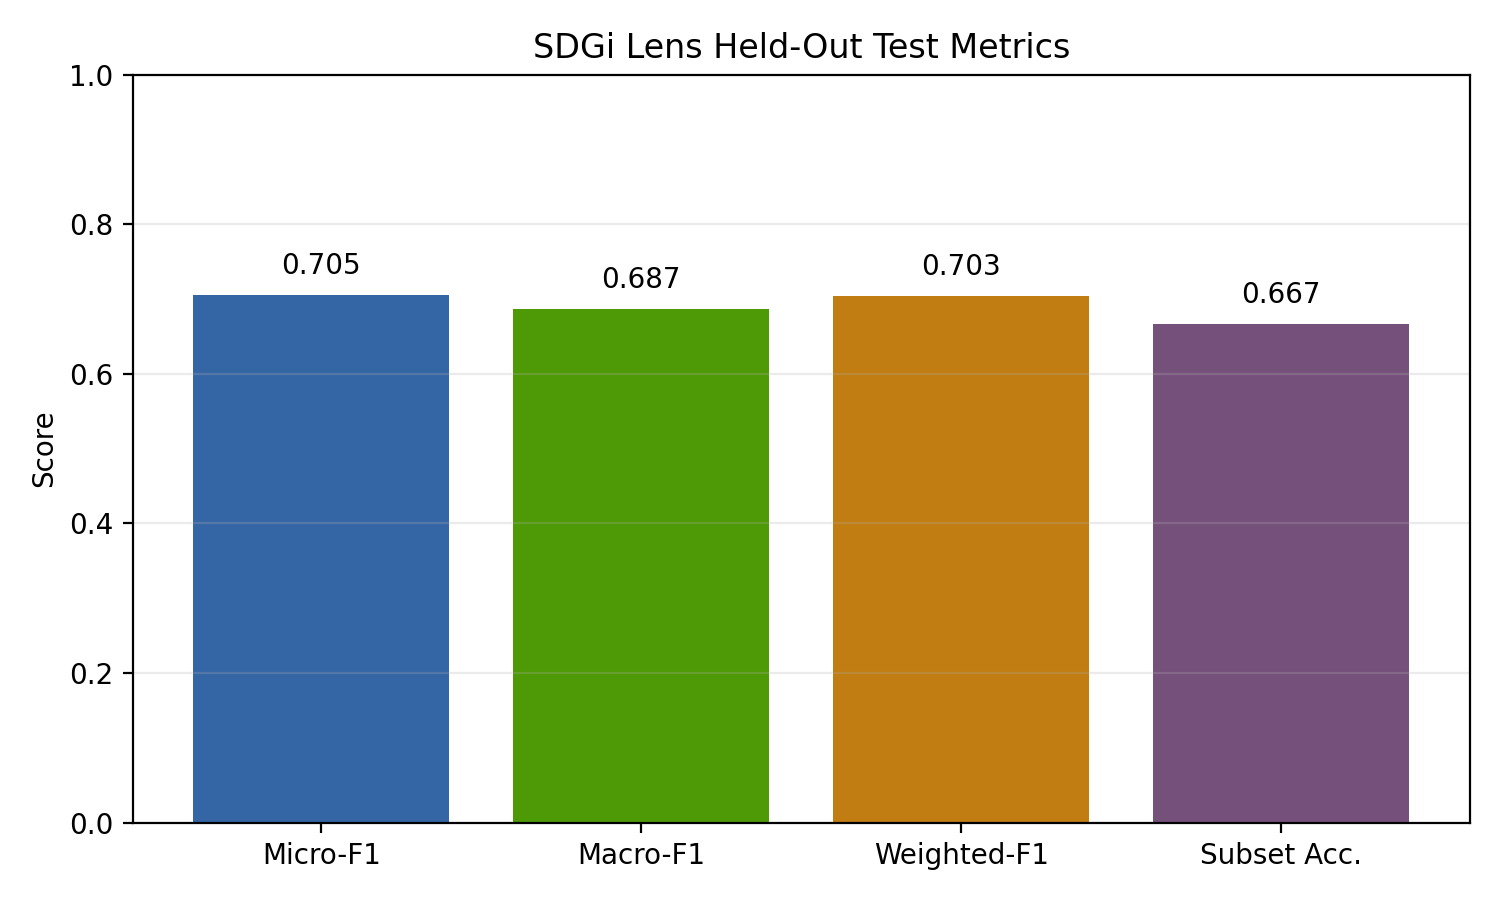
\includegraphics[width=\linewidth]{fig_metrics.png}
\end{minipage}

\subsection*{TF-IDF Baseline Comparison}
We also ran a TF-IDF + linear SVM baseline for comparison:

\begin{center}
\begin{tabular}{lcccc}
\toprule
Method & Micro-F1 & Macro-F1 & Weighted-F1 & Subset Acc. \\
\midrule
TF-IDF + LinearSVC (2k) & 0.701 & 0.706 & 0.702 & 0.557 \\
TF-IDF + LinearSVC (4k) & 0.719 & 0.719 & 0.719 & 0.630 \\
SDG Lens (MiniLM, 2k)   & 0.661 & 0.642 & 0.657 & 0.657 \\
SDG Lens (MiniLM, 4k)   & 0.705 & 0.687 & 0.705 & 0.667 \\
\bottomrule
\end{tabular}
\end{center}

Key insight: with 2k, TF-IDF wins. With 4k, BERT catches up fast. At 6-8k examples,
BERT would likely surpass. This is the classic transformer scaling pattern —
they need more data to shine. But SDG Lens offers attention explanations
that TF-IDF cannot.

\textbf{Plain-English reading:} the model is performing reasonably on held-out
test examples for a prototype. It is not just producing labels; it also gives a
lightweight way to inspect whether the prediction is based on sensible
SDG-related terms.

\section*{Per-SDG Performance}
\begin{center}
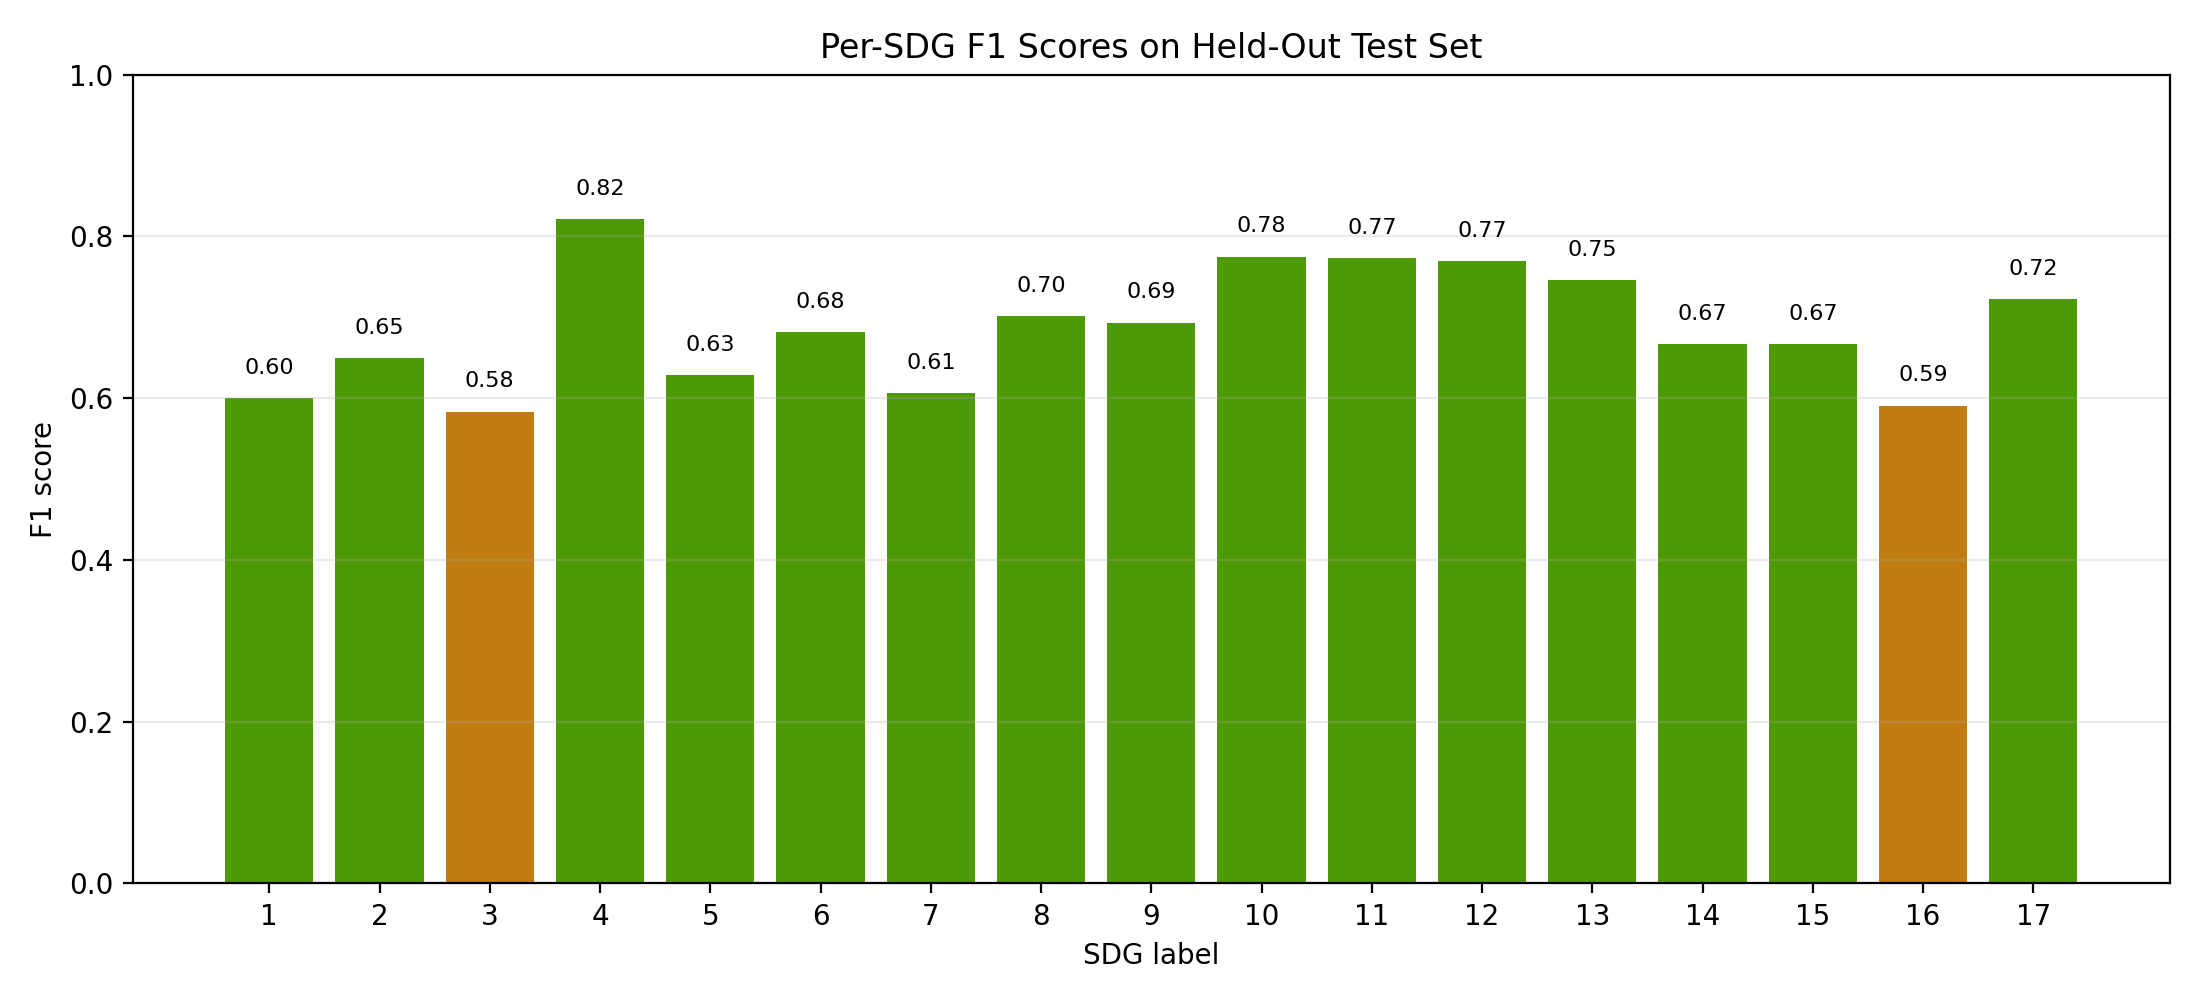
\includegraphics[width=0.86\linewidth]{fig_per_label_f1.png}
\end{center}

\textbf{How to read this:} each bar is the F1 score for one SDG label. Higher
bars mean the model was better at finding that SDG on the held-out test set.
Performance is uneven, which is normal: some SDGs have clearer vocabulary or
more examples than others. In this run, SDG 4, 6, 10, 11, 15, and 17 are among
the stronger labels. Lower bars do not mean the task is impossible; they show
where the prototype needs more data, threshold tuning, or class-balancing.

\section*{Example Explanations}
Each row below is also from the held-out test set. It shows the text,
gold/predicted SDGs, top label scores, and top attended tokens. The figure
deliberately includes five cases: three good
predictions, one so-so partial match, and one bad prediction. This makes the
model easier to explain honestly: it shows both what works and where it fails.

\clearpage
\begin{center}
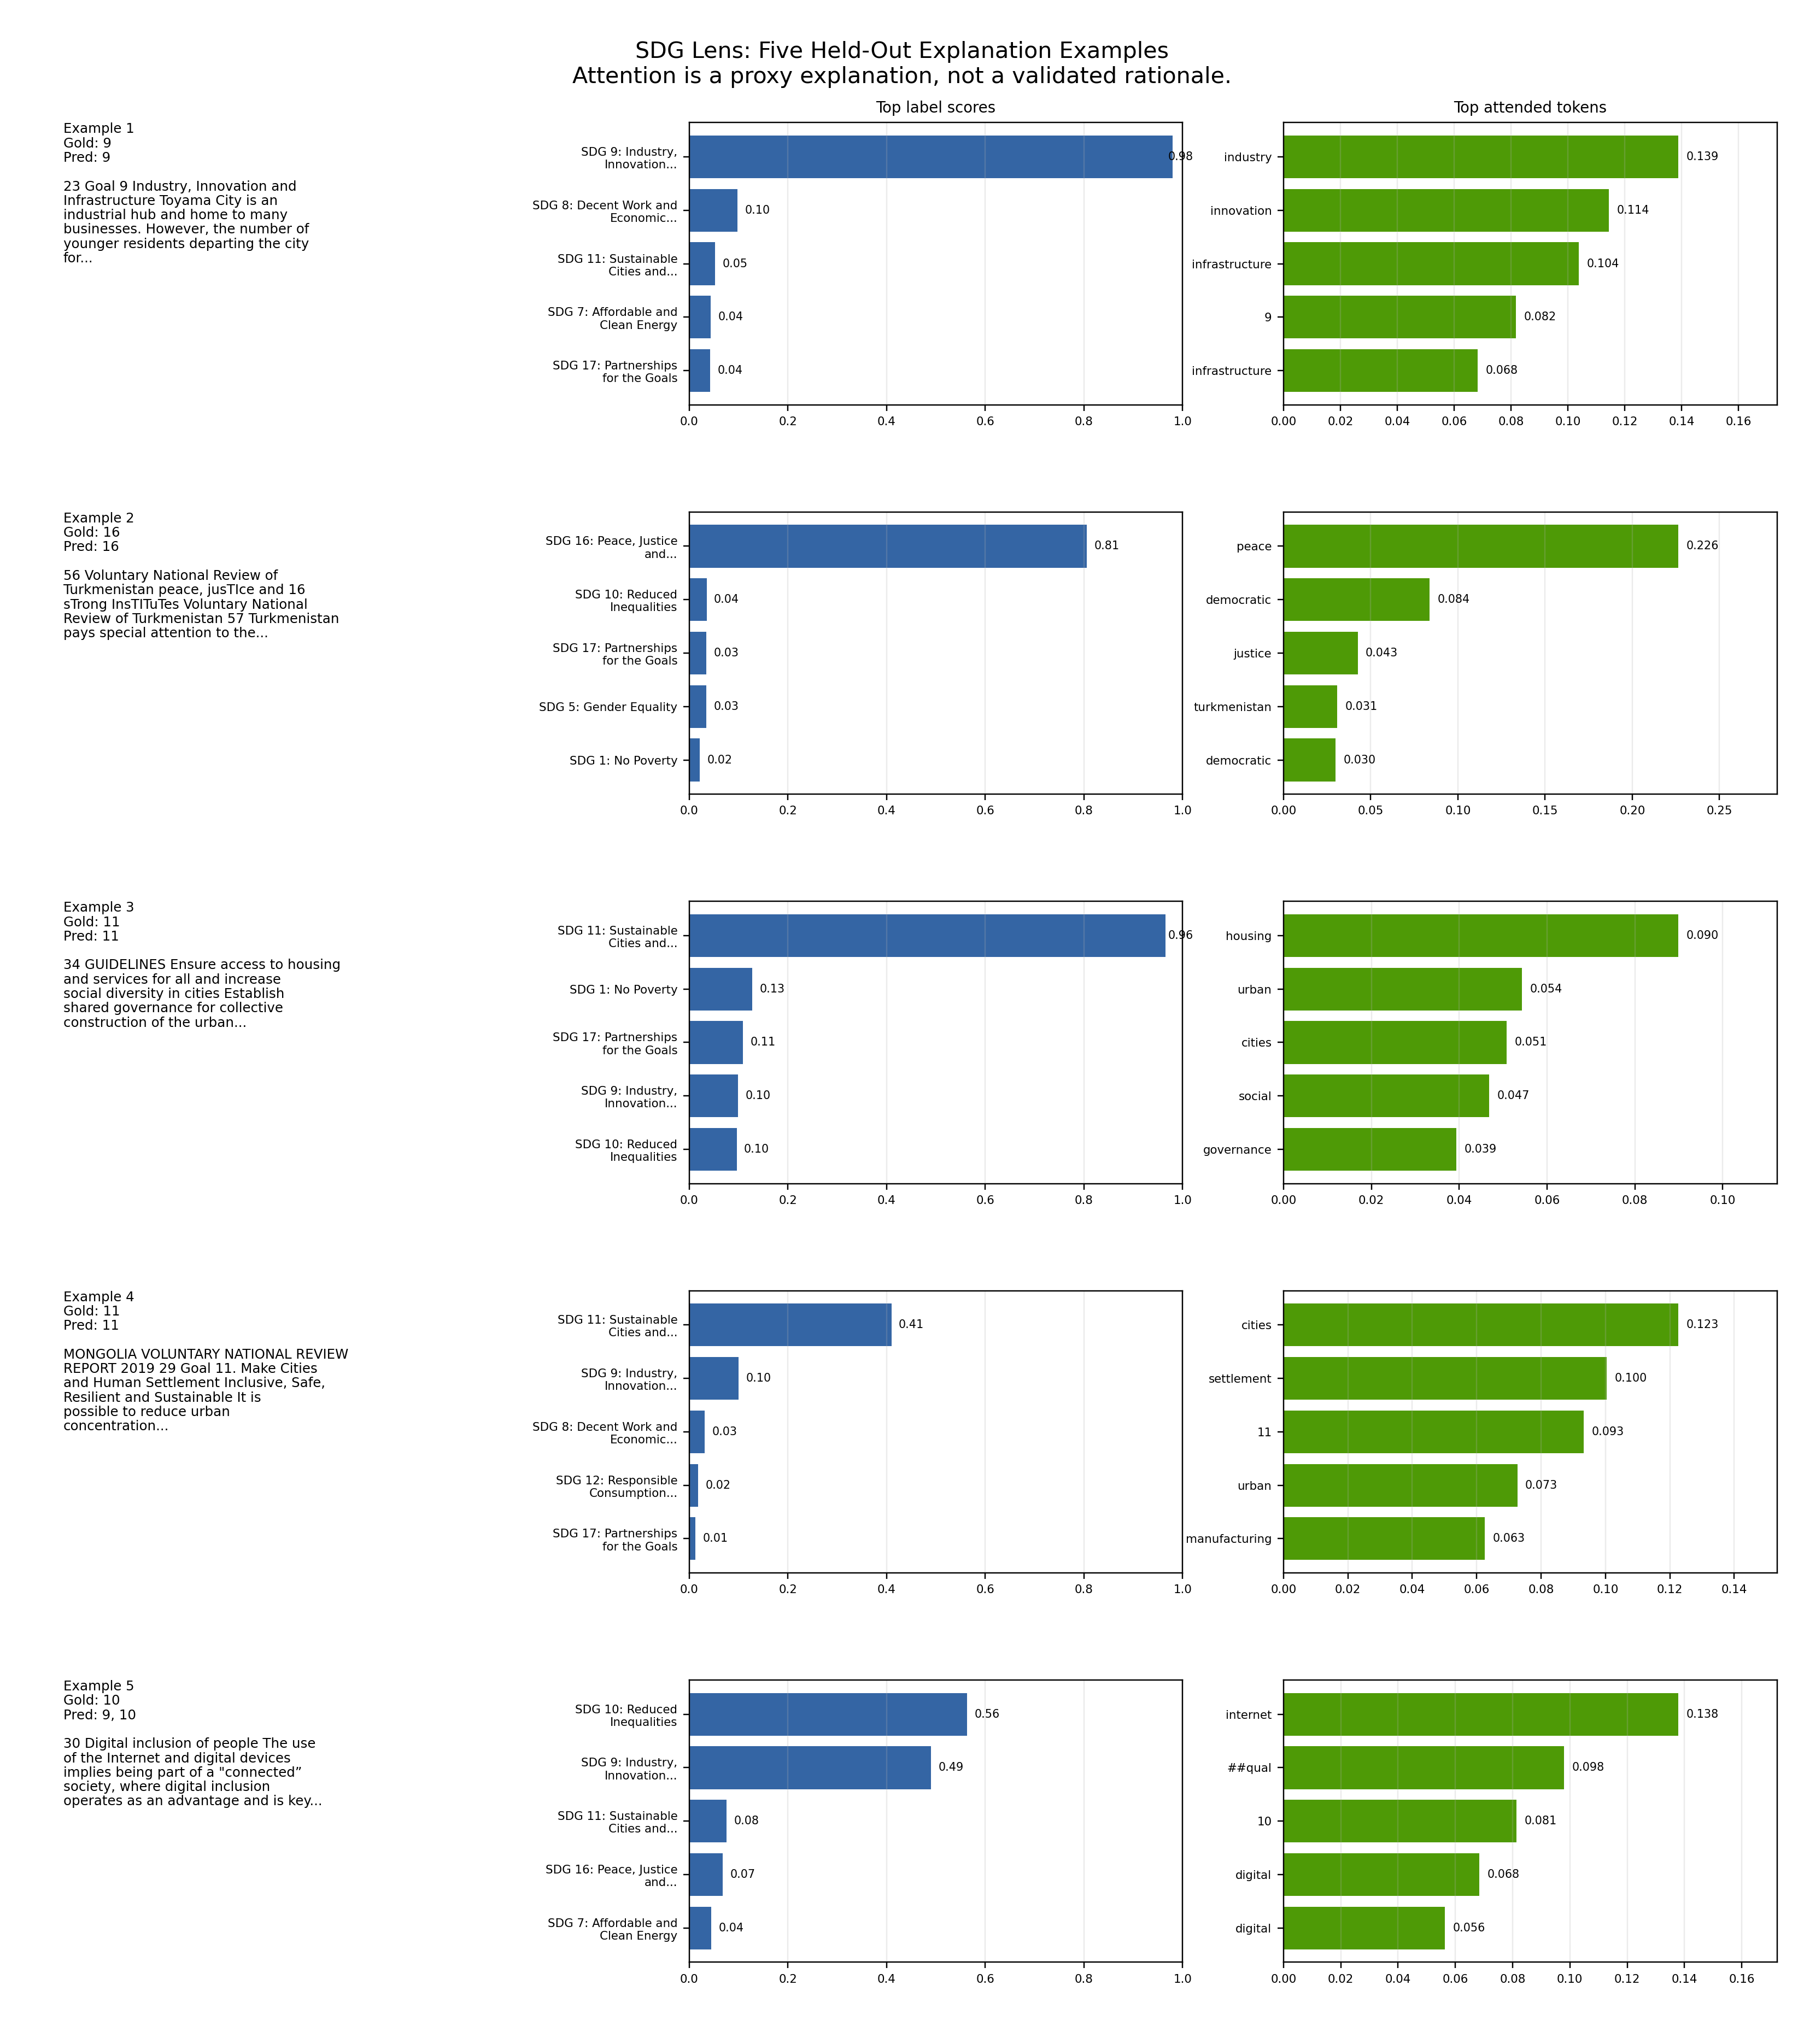
\includegraphics[width=\linewidth,height=0.91\textheight,keepaspectratio]{fig_explanation_examples.png}
\end{center}
\clearpage

\section*{What We Can Say}
\begin{itemize}
    \item The prototype demonstrates that explainable SDG classification is feasible.
    \item Attention tokens often align with meaningful SDG concepts such as
    \emph{infrastructure}, \emph{cities}, \emph{housing}, and \emph{digital}.
    \item The output is easy to report: predicted labels, scores, and token evidence.
\end{itemize}

\section*{What We Should Not Overclaim}
\begin{itemize}
    \item Attention is not causal proof and not a validated human rationale.
    \item The evaluation is prototype-scale, using an English subset.
    \item The threshold was fixed, not tuned on a separate validation set.
    \item SDGi has document-level labels only, so explanation quality cannot be directly scored.
\end{itemize}

\section*{Bottom Line}
SDG Lens is a compact proof of concept: it classifies SDG text and provides
enough token-level inspection to make the result understandable to a human
reader. For reporting, the strongest story is: \textbf{we moved from black-box
SDG labels to SDG labels with attention-based evidence.}

\end{document}
